\documentclass[12pt,conference]{IEEEtran}

% Add the compsoc option for Computer Society conferences.
%
% If IEEEtran.cls has not been installed into the LaTeX system files,
% manually specify the path to it like:
% \documentclass[conference]{../sty/IEEEtran}

\usepackage{amssymb, amsmath, amsthm}
\usepackage{graphicx, subfigure}
\usepackage{url, cite, verbatim}
\usepackage{booktabs}
\usepackage{xcolor}
\usepackage{nopageno}


\usepackage[ruled,vlined,linesnumbered]{algorithm2e}
%\newtheorem{algorithm}{Algorithm}
\newtheorem{assump}{Assumption}
\newtheorem{axiom}{Axiom}
\newtheorem{claim}{Claim}
\newtheorem{conj}{Conjecture}[section]
\newtheorem{crit}{Criterion}
\newtheorem{theorem}{Theorem}
\newtheorem{coro}{Corollary}[theorem]
%\newtheorem{coro}{Corollary}
\newtheorem{definition}{Definition}
\newtheorem{subsec:coding}{subsec:coding}
\newtheorem{fact}{Fact}
\newtheorem{hypo}{Hypothesis}
\newtheorem{lemma}{Lemma}
\newtheorem{obsv}{Observation}[theorem]
\newtheorem{prin}{Principle}
\newtheorem{prob}{Problem}
\newtheorem{ppty}{Property}
\newtheorem{propo}{Proposition}
\newtheorem{protocol}{Protocol}
\newtheorem{remark}{Remark}
\newtheorem{test}{Test}
\newtheorem{transform}{Conversion Algorithm}

\hyphenation{op-tical net-works semi-conduc-tor}

\newcommand{\ls}[1]  %% 1 in brackets means \ls takes 1 argument
   {\dimen0=\fontdimen6\the\font
    \lineskip=#1\dimen0
    \advance\lineskip.5\fontdimen5\the\font
    \advance\lineskip-\dimen0
    \lineskiplimit=.9\lineskip
    \baselineskip=\lineskip
    \advance\baselineskip\dimen0
    \normallineskip\lineskip
    \normallineskiplimit\lineskiplimit
    \normalbaselineskip\baselineskip
    \ignorespaces
   }
\newcommand{\reminder}[1]{{{\textcolor{red}{\bf (#1)}}}}


\begin{document}


\title{Human Activity Recognition Using Federated Learning}
 
\author{\IEEEauthorblockN{$^$Kushal Topnani, $^$Ahmad Mansoor Sajid, $^$Jitender Singh}
\IEEEauthorblockA{$^$Department of Computer Science, California State University, Sacramento, CA 95819, USA \\
$^$ktopnani@csus.edu, ahmadmansoorsajid@csus.edu, jitendersingh@csus.edu} 
}

\maketitle{}

\begin{abstract}

Today, smartphones have become an indispensable part of our lives. Without mobile phones, we cannot take over our lives. Since the advent of smartphones, there has been a revolution in the mobile communications industry. These days we use smartphones not only to make calls but to perform all day-to-day activities. They are most often used for entertainment purposes. The smartphone manufacturing company has loaded various sensors for the smartphone to improve the user experience. Two of these sensors are accelerometers and gyroscope. The accelerometer measures acceleration, while the gyroscope measures angular velocity. Here, we will try to use the data provided by the smartphone's accelerometer and gyroscope to classify the activities that the smartphone user is doing.

In this project, we have used the data set from UCI machine learning repository \cite{1dataset} and have used a federated learning model to predict the class of a particular activity given the accelerometer and gyroscope readings. We have also applied basic machine learning models to the given dataset, to compare the accuracy produced by the federated learning model and these base models. 

Human Activity Recognition (HAR) refers to the ability of machines to perceive human behavior. HAR is an important application of advanced machine learning and artificial intelligence technologies. These technologies use readings from various mobile sensors \cite{1dataset} to understand the semantic meaning of heterogeneous human behavior. This article presents a Federated learning method that can distinguish human actions based on data collected from actual human movements. Our data set is collected by the UCI ML repository, which uses the frequency and power characteristics of the collected human movement signals. This method will help to further study the biomedical signals based on human 
activity to identify it in a decentralized way.


\end{abstract}

%\begin{IEEEkeywords}
%HAR, Human Activity, Federated Learning, UCI, ML
%\end{IEEEkeywords}

\thispagestyle{plain}\pagestyle{plain}


\section{
\textbf{Introduction}
}

Human Activity Recognition (HAR) is a highly dynamic yet very important and challenging research topic with many applications in security, healthcare, smart environments, sports, robotics, and so on. HAR infers to the matter of learning and classification of human movements and activities from data collected from an individual or the surrounding environments of the individual. The form of the data can be inertial sensing measurements collected by smartphones, physical signals from sensors in wearable devices, or vision-based information like images, audio, and video data collected from environmental devices.

Computer vision-based methods have broadly been used for human activity recognition and tracking, but those methods generally require infrastructure support, for example, installation of video cameras, GPS, or Leap Motion devices \cite{2leap} in the monitoring areas \cite{3poppe2010survey},\cite{4Jaouedi2016HumanAR} to identify activities of a person. Alternatively, a more efficient method is to process the data from inertial measurement sensors built in a user’s smartphone \cite{5kwapisz2011activity},\cite{6kwapisz2010cell}, or on wearable sensory devices worn on a user’s body \cite{7casale2011human},\cite{8krishnan2008real} to track the user’s motion.

The main aims of HAR systems are to perceive and identify human activities and to classify ongoing movements effectively. There are numerous application domains for HAR where concepts are researched, and effective systems are developed. HAR systems are divided roughly into four categories and application areas \cite{9ranasinghe2016review}: Active and Assisted Living (AAL) systems for smart homes, healthcare monitoring applications, monitoring and security surveillance systems for indoor and outdoor activities, and Tele-Immersion (TI) applications for gaming and healthcare. The purpose of AAL systems is to provide proper technical support for specifically elderly people to live independently in their homes. Advancements in this field \cite{10menschner2011reaching} focuses on the increasing need for care and support for older people. According to \cite{11demiris2008senior}, a smart home is an environment equipped with sensors that enhance the safety of residents and monitor their health conditions. The HAR system, to be able to provide such support, needs to collect and analyze information through either a smartphone’s inertial measurement sensors or wearable sensor devices.

Monitoring systems for healthcare are developed based on one or a combination of multiple components of activity recognition models such as fall detection, activity tracking, security alarm, intellectual assistance, and so on. Most of the healthcare systems use wearable sensors devices like E-safe fall detection and notification system \cite{12gannapathy2013zigbee} which detects and notifies the relevant responders of the fall of the patient using ZigBee-based wearable sensor technology. Also, another study in \cite{13ogbuabor2018human} has investigated the effectiveness of smartphone sensors explicitly accelerometer and gyroscope sensors for healthcare systems. Similarly, HAR is also used in TI systems to track and simulate human activities and behaviors in a virtual environment to build interactive game interfaces or to increase the efficiency of communication means.
The increase in usage and sophistication of mobile devices, and growth of its computing resources, such as processing, portability, connectivity, and its power of sensing such as motion, audio, image, location, temperature, direction, and acceleration, have attracted researchers to find innovative solutions for HAR.
Researchers have categorized human activities into four categories based on different parts of the body being engaged in the action and their complexity \cite{14aggarwal2011human}: \newline

•	Gesture: It is a visible bodily action representing a specific message. It is a movement made with the hands, face or other parts of the body such as Okay gestures and thumbs up. \newline

•	Action: Which is a set of physical movements conducted by only one person like walking and running. \newline

•	Interactions: It is a set of actions executed by at most two actors. At least one subject is a person and the other one can be a human or an object (handshaking, chatting, etc). \newline

•   Group activities: It is a mixture of gestures, actions, or interactions. The number of performers is at least two plus one or more interactive objects (playing volleyball, obstacle racing, etc). \newline

HAR is a classification machine learning task, and its purpose is to learn the activity performed by a person. Activities can be of different types such as walking, standing, sitting, lying, or running. Machine learning models are trained on sensor data from accelerometer and gyroscope sensors in smartphones or other wearable sensing devices to identify activities. Researchers have developed different deep learning models and achieved highly accurate results for HAR tasks on the data collected from smartphones \cite{4Jaouedi2016HumanAR},\cite{6kwapisz2010cell}-\cite{7casale2011human}, \cite{15yao2017deepsense},\cite{16ordonez2016deep},\cite{17hammerla2016deep}. Yao et al.\cite{14aggarwal2011human} proposed a deep learning model trained on accelerometer and gyroscope mobile sensor data which is consisted of a combination of a Recurrent Neural Network (RNN) and a Convolutional Neural Network (CNN). For this model, clients need to send a lot of data to a cluster or a centralized server for interpretation and training, which is a challenging task due to communication costs and user privacy issues.

To address the challenges, in separate research, McMahan et al. \cite{18mcmahan2016federated} proposed using federated learning to train the classifier. Federated learning is a distributed model which permits building a global model and keeping the sensor data with the user. This algorithm ensures that the privacy of the user is preserved and that the communication incurs lower cost as the data interpretation and training takes place at the user’s device. To classify and recognize activities with accuracy, a lot of sensor data is required to be collected. Though federated learning is the solution to train the classifier, the algorithm is not much practiced, and the application environments are not very well known.

In this project, we implement federated learning to train a HAR classifier and evaluate its performance. We will also compare HAR classifier results trained using state-of-the-art centralized learning, specifically, Logistic Regression \cite{19zaki2020logistic}, Random Forest \cite{20feng2015random}, and Decision Tree \cite{21fan2013human}, where the classifier is trained on sensor data stored in a central server, with HAR classifier results trained using federated learning. Both methods (centralized and distributed) are evaluated using two different models: (1) a softmax regression model, and (2) a Deep Neural Network (DNN) model.

The main contribution of our paper is that we have trained both models in two ways, using centralized learning and federated learning on a HAR dataset with 3-axial linear acceleration and 3-axial angular velocity data. We have also evaluated and compared the performance of the logistic regression, random forest, and decision tree algorithms trained with federated learning compared to the algorithms trained with centralized learning and demonstrate that federated learning offers acceptable accuracy, in certain environments, by training and utilization of the models for HAR.

The rest of the paper is organized as follows. In section II we provide some background on machine learning and federated learning and some related work on HAR. Section III presents the dataset we have used and our experimental and evaluation setting. In section V we introduce the models and the algorithms we trained for HAR. Then, in section VII results and evaluations are presented. Finally, our work is concluded in section VIII and we provide some future work.  

\section{
\textbf{Background and Related Work}
}

Machine learning is the study of algorithms and a data analysis method that improves automatically through experience and using data. Its goal is to induce a prediction decision model or classification decision model from data that will be able to make automatic decisions on new data. Some patterns cannot be programmed explicitly whose exact description is not known as they might be hidden within huge datasets. Machine learning algorithms will find and identify such patterns and will train the models. The HAR classification task is to predict different human activities based on a set of sensors worn or used by the user. This set of sensors consist of tri-axial accelerometer and gyroscope sensors. The accelerometer is a sensor that measures acceleration forces like counting steps, and a gyroscope sensor measures the screen rotation or angular velocity of a device.
In comparison to state-of-the-art classical machine learning models, deep learning models have the advantage of using large datasets, and the feature extraction process is not used with deep learning models. The learning in federated learning is performed by a federation of devices that produces training data. In centralized learnings, the training data gets stored in a central server. The main goal of federated learning is to train a model by using a subset of clients from a set of all clients, each client having its dataset. The local models are getting trained with specific methods in several epochs and the results are synchronized with the server that holds the global model. The server collects updates from all clients after the local models are trained. We have used two evaluation metrics for global updates, first when the local models are getting updated only once by the client, and second when the local models are getting updated by the client multiple times. There are two main advantages of using federated learning algorithm (distributed) over using the centralized learning algorithms, (1) all client-specific and sensitive data remain on the client’s device, and (2) the communication cost between client and server is reduced as clients do not contact the server to train each bit of data, instead of synchronous updates are sent to the server at the end of each training epochs.

The study of HAR is an important research direction with various practical applications in healthcare, fall detection, TI, and others. Different machine learning and deep learning-based methods are developed to address issues in HAR and achieved effective results \cite{22chen2019towards}. wearable and smartphone sensors based on human activity recognition utilizes wearable devices or smartphones to monitor and obtain on-body sensors data with the accelerometer, magnetometer, and gyroscope sensors \cite{23gupta2014feature}. For example, Lee and Mase \cite{24lee2002activity} used the acceleration and angular velocity sensor data measured by wearable devices, to determine the users’ location information and identify their sitting, standing, and walking behaviors. Mantyjarvi et al. \cite{25mantyjarvi2001recognizing} utilized the independent component analysis and principal component analysis schemes to recognize one person’s walking posture based on the acceleration data collected from the smartphone placed into the user’s waist. The results show that activity recognition methods based on wearable and smartphone sensors work effectively for the recognition tasks for complex activity recognition. 



\section{
\textbf{Data set}
}

“Human Activity Recognition Using Smartphones Data Set” was chosen for the project, a multivariate time-series based dataset of 10299 instances built from the recordings of 30 subjects performing daily-life activities(ADL) while carrying a waist-mounted smartphone with embedded inertial sensors, with emphasis on the output task of Classification or Clustering. The experiments have been carried out with a group of 30 volunteers within an age bracket of 19-48 years. Each person performed six activities ( WALKING, WALKING\_UPSTAIRS, WALKING\_DOWNSTAIRS, SITTING, STANDING, LAYING ) wearing a smartphone on the waist. Using its embedded accelerometer and gyroscope, we captured 3-axial linear acceleration and 3-axial angular velocity at a constant rate of 50Hz. The experiments have been video-recorded to label the data manually. The obtained dataset has been randomly partitioned into two sets, where 70\% of the volunteers were selected for generating the training data and 30\% the test data.

The sensor signals (accelerometer and gyroscope) were pre-processed by applying noise filters and then sampled in fixed-width sliding windows of 2.56 sec and 50\% overlap (128 readings/window). The sensor acceleration signal, which has gravitational and body motion components, was separated using a Butterworth low-pass filter into body acceleration and gravity. The gravitational force is assumed to have only low frequency components, therefore a filter with 0.3 Hz cutoff frequency was used. From each window, a vector of features was obtained by calculating variables from the time and frequency domain. These activities are encoded as follows:\\

WALKING-- 1 \\
WALKING\_UPSTAIRS-- 2 \\
WALKING\_DOWNSTAIRS-- 3 \\
SITTING-- 4 \\
STANDING-- 5 \\
LYING-- 6 \\

Triaxial acceleration from the accelerometer (total acceleration) and the estimated body acceleration.
Triaxial Angular velocity from the gyroscope.
A 561-feature vector with time and frequency domain variables. Its activity label. An identifier of the subject who carried out the experiment.

Accelerometer readings are divided into gravity acceleration and body acceleration readings, which has x, y and z components each. Gyroscope readings are the measure of angular velocities which has x, y and z components.Jerk signals are calculated for Body-Acceleration readings.
Fourier Transforms are made on the above time readings to obtain frequency readings.
Now, on all the base signal readings., mean, max, mad, sma, arcoefficient, energy-bands, entropy etc., are calculated for each window.
Extra features are calculated by taking the average of signals in a single window sample. These are used on the angle() variable.
Finally, we got feature vector of 561 features and these features are given in the dataset.
Each window of readings is a data-point of 561 features.


\section{
\textbf{Problem Statement}
}

Domain experts from the field of Signal Processing collects the data from Accelerometer and Gyroscope of Smartphone. They break up the data in the time window of 2.56 seconds with 50\% overlapping i.e., 128 reading. They engineered 561 features from each time window of 2.56 seconds. By using either human engineered 561 feature data or raw features of 128 reading, our goal is to predict one of the six activities that a Smartphone user is performing at that 2.56 Seconds time window.
\newline \\
\\
\emph{By using either human engineered 561 feature data or raw features of 128 reading, our goal is to predict one of the six activities that a Smartphone user is performing at that 2.56 Seconds time window.}


\section{
\textbf{Our Methodology}\label{sec:sys}
}

Human Activity Recognition is a multi-class classification problem, which belongs to the scope of "human activity recognition" through joint learning. A high degree of recognition of human activities offers different advantages. Portable health applications may become a trap for the elderly and be infected, which can quickly recover from any injury or prevent misfortune. This data set is useful for us because today everyone has a smartphone and controls their health through the apps they can access. Our goal is to build a powerful and basic federated learning model that can accurately predict a person’s exercises in a day, depending on the sensor information they have access to. Compared with the centralized model, federated learning has different points of interest, but our main focus here is the privacy issues collected by private sensor information accessible on the customer's smartphone. We intend to build a model to train the private information in the client frame and transfer the weights to the global model to predict and evaluate the public data set.

We have also used classic machine learning algorithms for the same data set. These algorithms predicted the class of the activities which will help us in evaluating the federated learning model.


% \subsection{Data Exploration}


\begin{figure} [!t]
	\centering
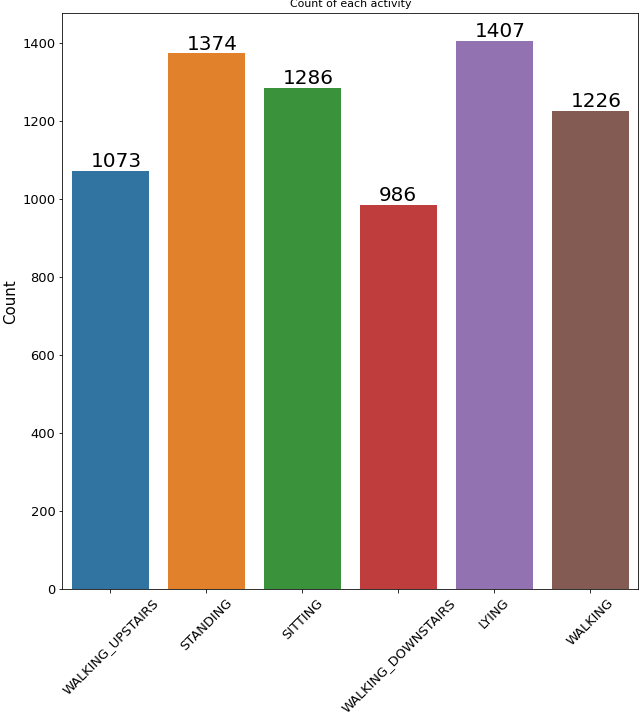
\includegraphics[width=3.1in]{EDA.PNG}
	\caption{Count of each activity}
	%\vspace{-0.1in}
	\label{Number of each activity}
	%\vspace{-0.1in}
\end{figure}

\section{
\textbf{Design}\label{sec:e}
}

In this section, we narrate the design, training system, and implementation of Federated learning, solve this classification problem. We will also discuss the base machine learning models which will be used to compare the performance of the federated learning model.

\subsection{Federated Learning}

Standard machine learning approaches require centralizing the training data on one machine or in a data center. Federated learning is a secure and robust cloud infrastructure for processing this data to make our services better. Now for models trained from user interaction with mobile devices.
Federated Learning enables mobile phones to collaboratively learn a shared prediction model while keeping all the training data on the device, decoupling the ability to do machine learning from the need to store the data in the cloud. This goes beyond the use of local models that make predictions on mobile devices by bringing model training to the device as well.

The device downloads the current model improves it by learning from data on your phone and then summarizes the changes as a small focused update. Only this update to the model is sent to the cloud, using encrypted communication, where it is immediately averaged with other user updates to improve the shared model. All the training data remains on the users' devices, and no individual updates are stored in the cloud.
We have divided the data set into three different section. Each section will be used to train different models imitating the local learning at the device. After training the three models, we have transferred the learning to a global model. Testing data has been used to compute the accuracy of this global model.

Figures 2 and 3 show the learning curves of accuracy and loss for one of the three models that we have trained to simulate the federated learning. 
In federated learning, the test accuracy and loss measures for servers are reported after the aggregation of the epochs while for the clients the accuracy and loss measures are evaluated before sending to the server.

\begin{figure} [!t]
	\centering
	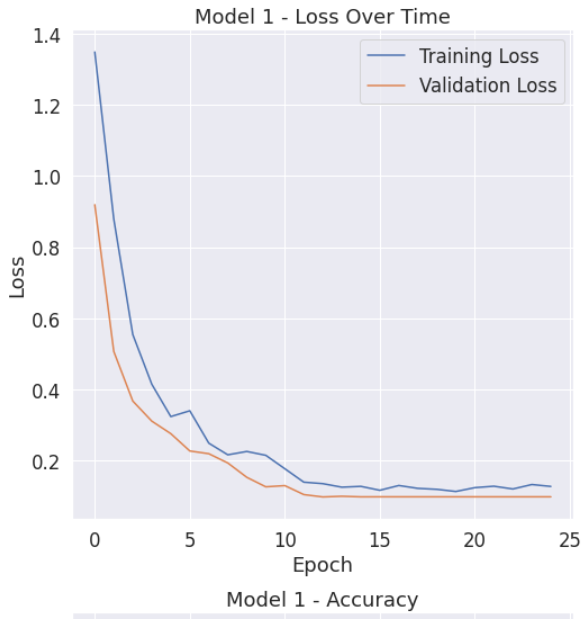
\includegraphics[width=3.1in]{Model_1_loss.PNG}
	\caption{Learning curve(Loss) federated learning model-1}
	%\vspace{-0.1in}
	\label{Learning curve for LoT of federated learning model-1}
	%\vspace{-0.1in}
\end{figure}

\begin{figure} [!t]
	\centering
	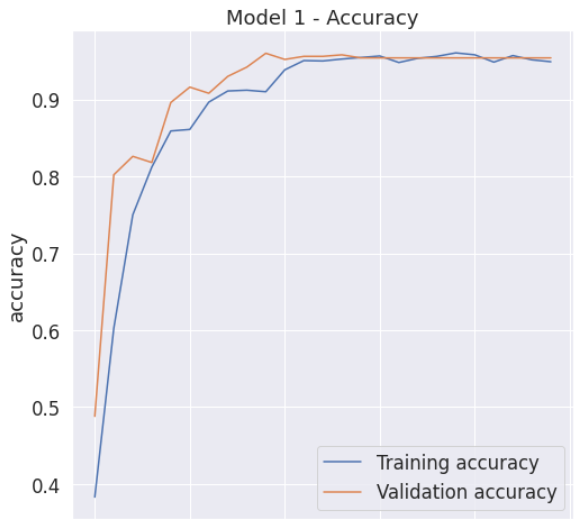
\includegraphics[width=3.1in]{model1_accuracy.PNG}
	\caption{Learning curve(Accuracy) of federated learning model-1}
	%\vspace{-0.1in}
	\label{Learning curve for the accuracy of federated learning model-1}
	%\vspace{-0.1in}
\end{figure}

\subsection{Logistic Regression}

The logistic regression model can be used in various fields including machine learning, most medical fields, and many social sciences. The outcome received in logistic regression is a dependent variable and it's continuous which helps in finding 1 out of an infinite number of possible variables. It can help helpful in finding out the email is spam or not spam, etc., the logistic function to map the input variable to categorical dependent variable. Unlike other regression, logistic regression gives only binary outcomes.

\subsection{SVM}

Linear Support Vector Machine is a supervised machine learning technique which can be used in classification or regression problem. To improve the quality of the prediction SVM uses an additional vector for inseparable data. This is quite an improvement over the other classifier as it can be used for both linear and non-linear decision boundaries. The SVM uses the kernel function to make a decision and separate boundaries. Support Vector Machines are quite an improvement over the maximal margin algorithm.

\subsection{Decision Tree}

Decision tree learning is one of the predictive model techniques used in statistics, data mining, and machine learning application. Uses the concept of observation and target value where observation represents the branches and target value represents leaves node which shows the result value. The relation between the labels and branches is like that the target value can be used as a classification tree where leaves annotate the labels and branches while conjunction of feature gives the leading toward the class labels one of the predictive modeling approaches used in statistic, data mining and machine learning.


\section{
\textbf{Results}
}

In this section, we present the results of using federated learning for the task of HAR. We have trained classic machine learning models training on one dataset where all sensor data is available and one federated learning with three different data distributions across clients in federated learning. We evaluate federated learning for HAR in terms of accuracy and confusion matrix.

We selected our baseline accurate performing models for a comparison between models trained using federated learning on all data and centralized learning. Using mean accuracy level, we recognized and rated the 3 models we used centralized learning to train, and the global model trained with federated learning.

\begin{table}[!t]
\caption{Accuracy for different models}
\begin{center}
\begin{tabular}{c|cccc}
\toprule %\hline
\textbf{Models} & \textbf{\textit{Accuracy}} \\
\midrule %\hline
Logistic Regression& 96.1\% \\
%\hline
Linear SVM& 96.4\% \\
%\hline
Decision Tree& 87\% \\
%\hline
Global Model(Federated)& 88.8\% \\
\bottomrule %\hline
\end{tabular}
\label{tab1}
\end{center}
\vspace{-0.1in}
\end{table}

Table 1 depicts classification accuracy of the 3 models of centralized learning versus the global model of federated learning.

\subsection{Logistic Regression}

For centralized training approach, the logistic regression algorithm was able to reach an accuracy of 96.1\%, which is in the upper scale of the state-of-
the-art centralized learning results. Figures 4, 5, and 6 describes the confusion, recall, and precision matrices for the logistic regression algorithm.

\begin{figure} [!t]
	\centering
	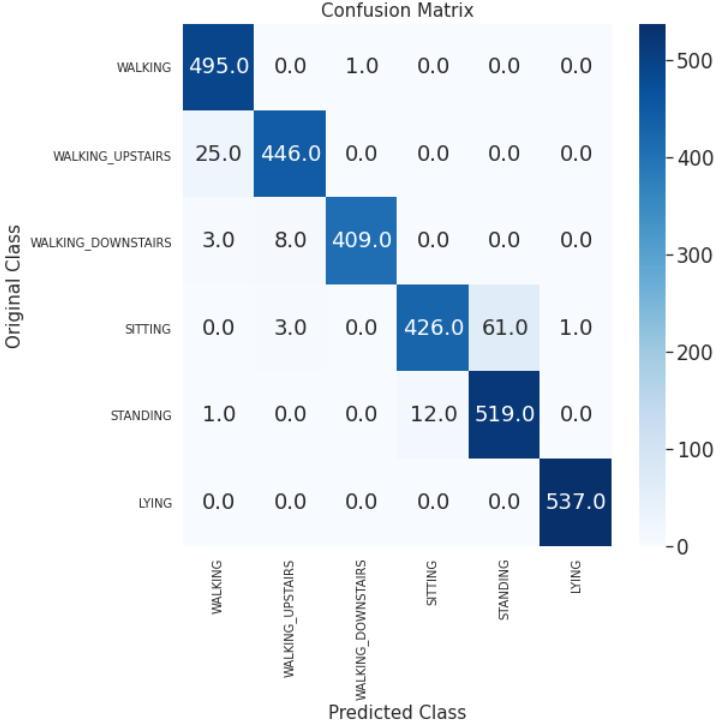
\includegraphics[width=3.1in]{Logistic_cm.PNG}
	\caption{Logistic Regression confusion Matrix}
	%\vspace{-0.1in}
	\label{}
	%\vspace{-0.1in}
\end{figure}

\begin{figure} [!t]
	\centering
	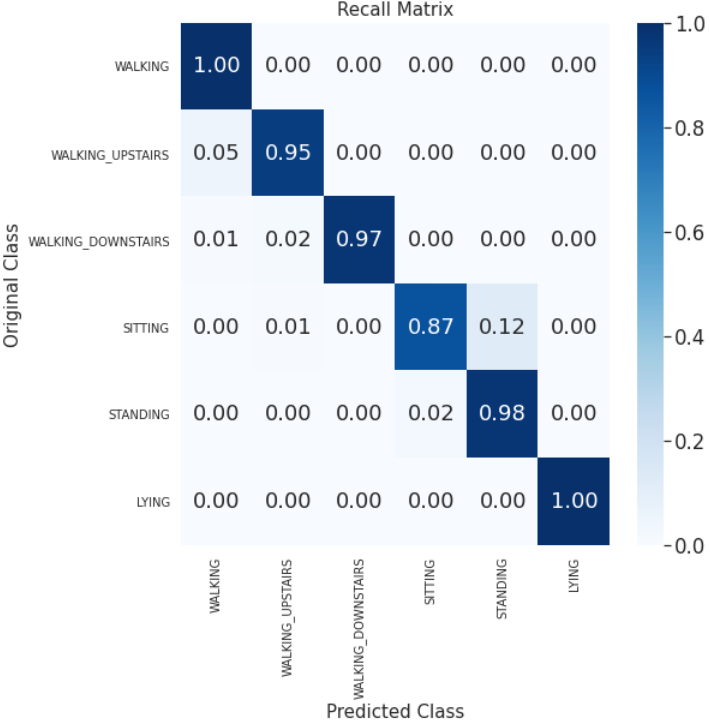
\includegraphics[width=3.1in]{Logistic_recall.PNG}
	\caption{Logistic Regression Recall Matrix}
	%\vspace{-0.1in}
	\label{}
	%\vspace{-0.1in}
\end{figure}

\begin{figure} [!t]
	\centering
	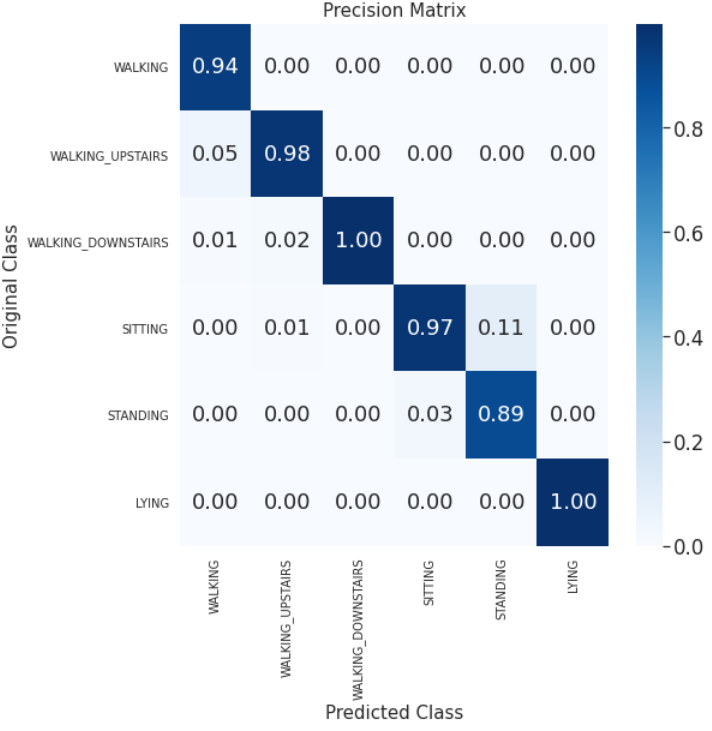
\includegraphics[width=3.1in]{Logistiv_pm.PNG}
	\caption{Logistic Regression precision Matrix}
	%\vspace{-0.1in}
	\label{}
	%\vspace{-0.1in}
\end{figure}

\subsection{Support Vector Machine}
The only method better than the logistic regression in our experiment was the SVM algorithm with 96.4\% classification accuracy. The confusion, recall, and precision matrices for SVM are plotted in Figures 7 through 9. 

\begin{figure} [!t]
	\centering
	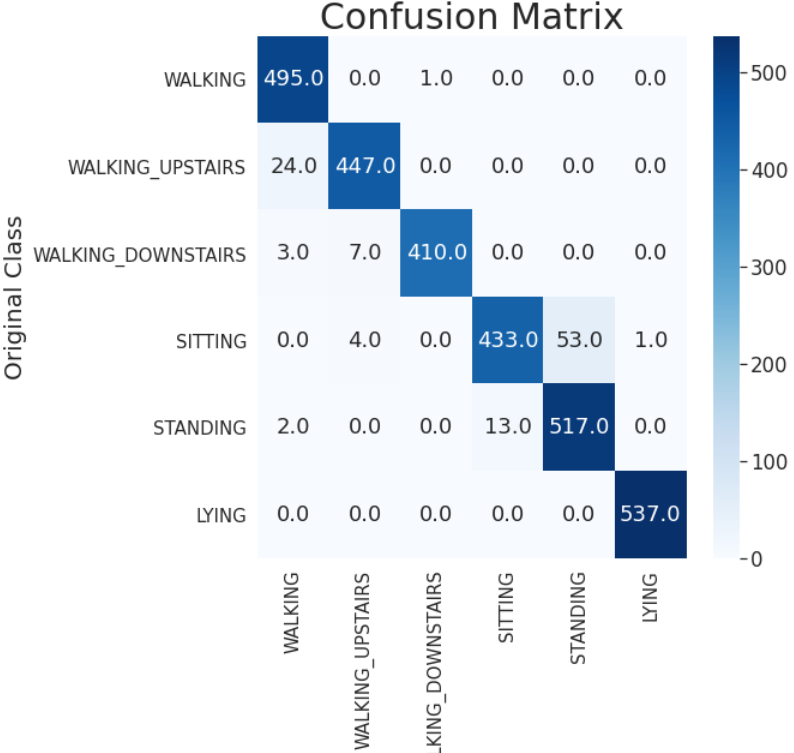
\includegraphics[width=3.1in]{svm_cm.PNG}
	\caption{SVM Confusion Matrix}
	%\vspace{-0.1in}
	\label{}
	%\vspace{-0.1in}
\end{figure}
\begin{figure} [!t]
	\centering
	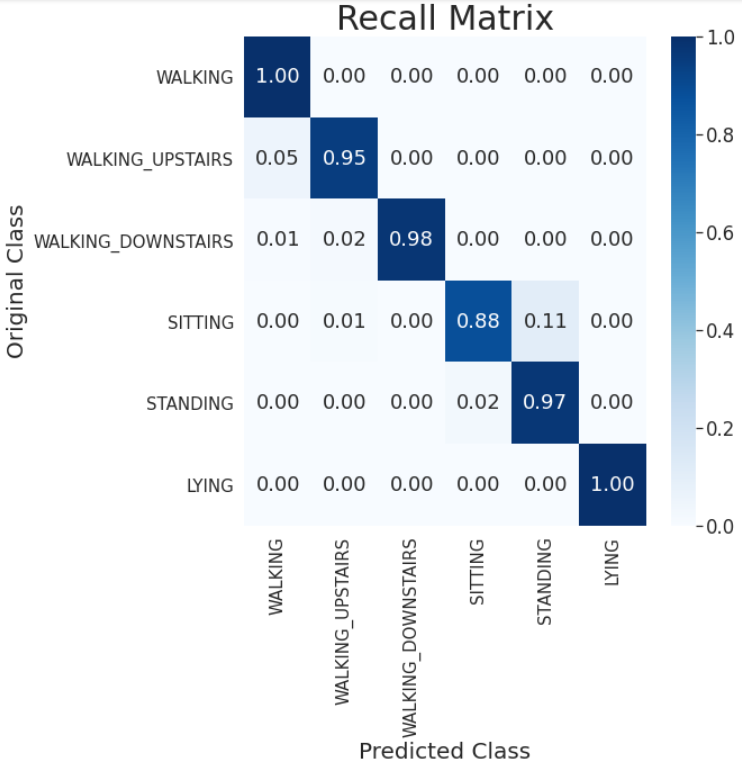
\includegraphics[width=3.1in]{svm_recall.PNG}
	\caption{SVM Recall Matrix}
	%\vspace{-0.1in}
	\label{}
	%\vspace{-0.1in}
\end{figure}

\begin{figure} [!t]
	\centering
	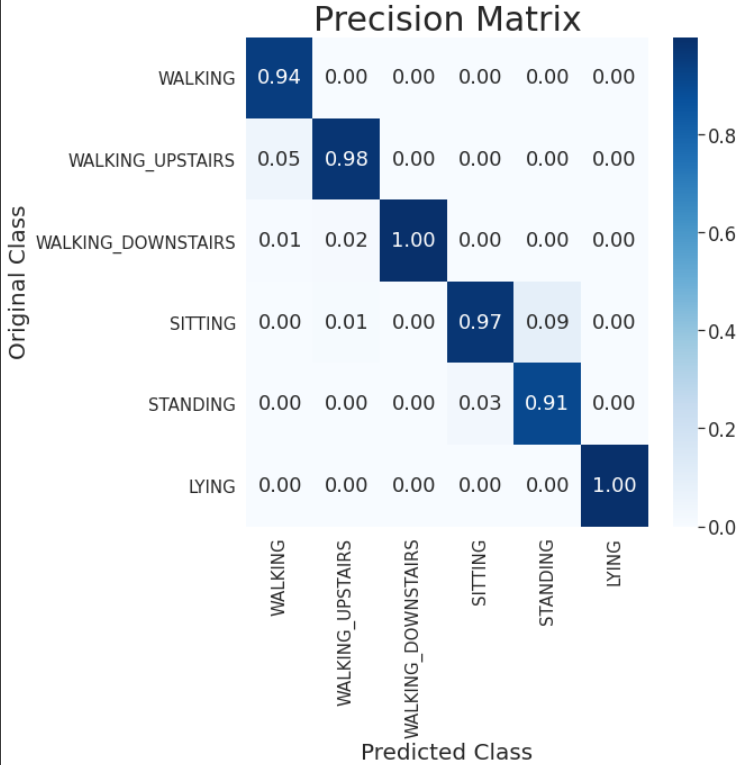
\includegraphics[width=3.1in]{svm_pm.PNG}
	\caption{SVM Precision Matrix}
	%\vspace{-0.1in}
	\label{}
	%\vspace{-0.1in}
\end{figure}

\subsection{Decision Tree}
The decision tree algorithm trained on centralized learning model resulted in the lowest classification accuracy among all other centralized models as well as the global (federated) model with accuracy level of 87\%. We can also notice the difference in its confusion, recall, and precision matrices plotted in figures 10 through 12.\\

\begin{figure} [!t]
	\centering
	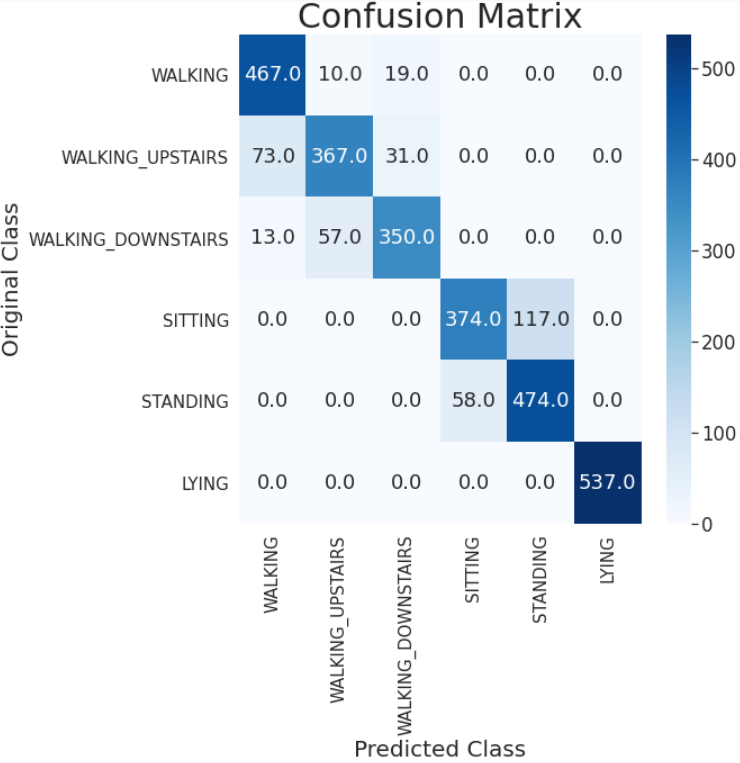
\includegraphics[width=3.1in]{tree_cm.PNG}
	\caption{Decision Tree Confusion Matrix}
	%\vspace{-0.1in}
	\label{}
	%\vspace{-0.1in}
\end{figure}
\begin{figure} [!t]
	\centering
	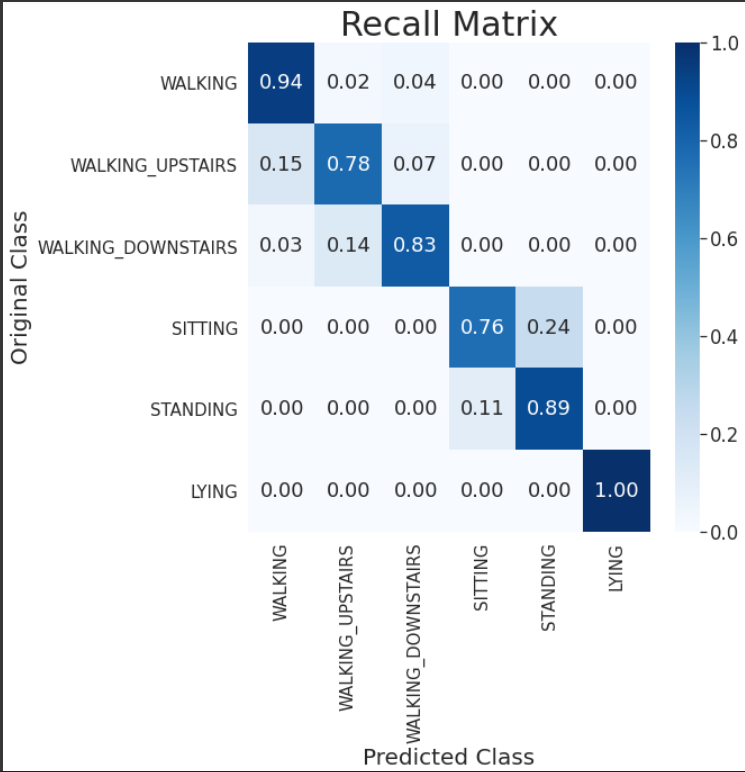
\includegraphics[width=3.1in]{tree_recall.PNG}
	\caption{Decision Tree Recall Matrix}
	%\vspace{-0.1in}
	\label{}
	%\vspace{-0.1in}
\end{figure}
\begin{figure} [!t]
	\centering
	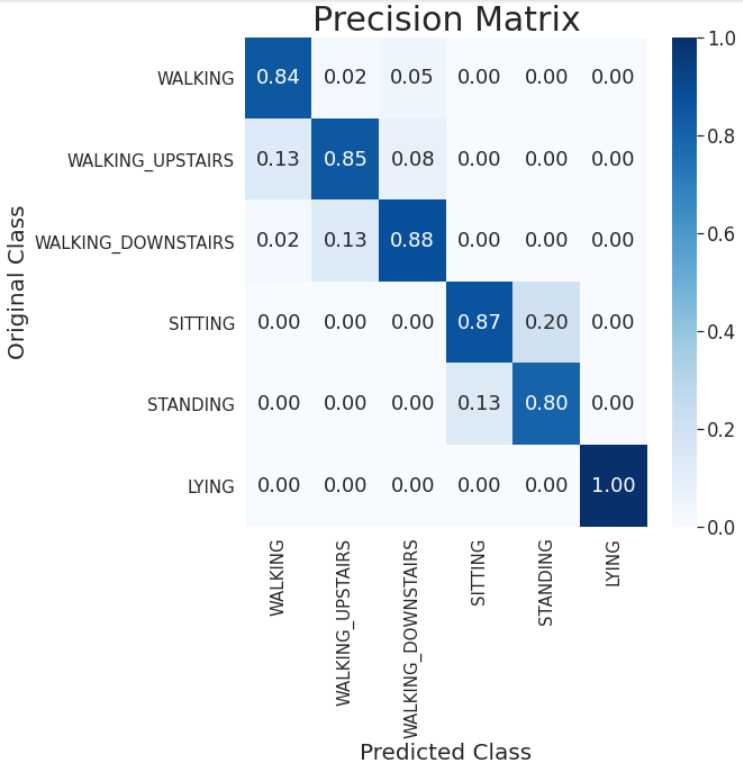
\includegraphics[width=3.1in]{tree_pm.PNG}
	\caption{Decision Tree Precision Matrix}
	%\vspace{-0.1in}
	\label{}
	%\vspace{-0.1in}
\end{figure}

\begin{figure} [!t]
	\centering
	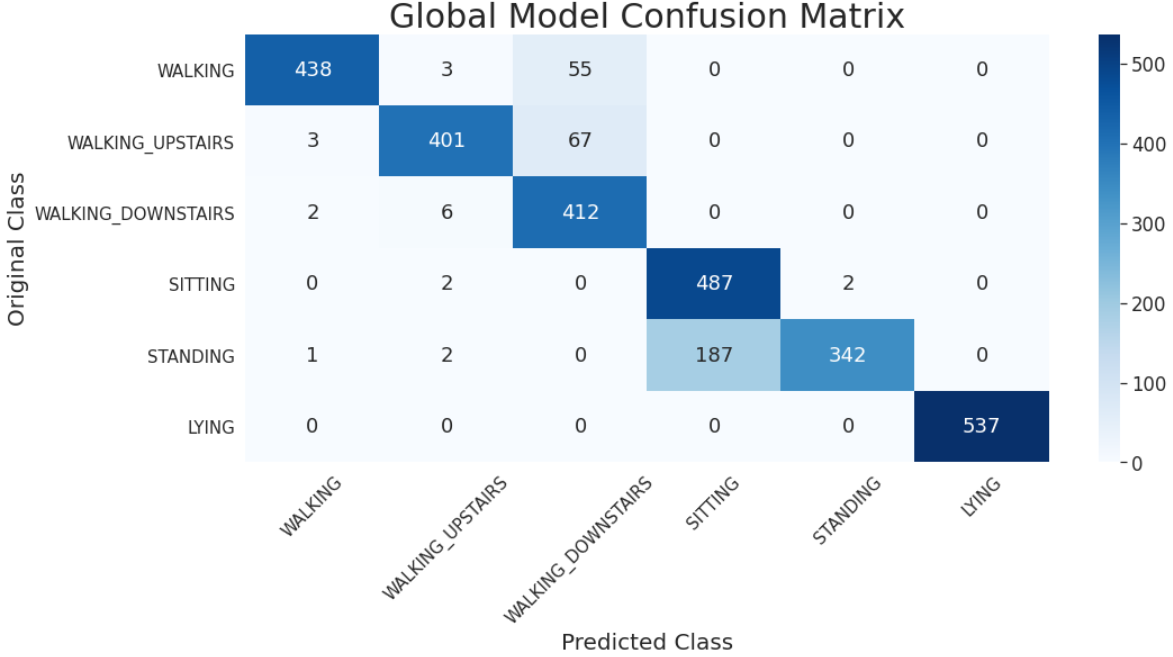
\includegraphics[width=3.1in]{global_cm.PNG}
	\caption{Global Model(Federated Learning) Confusion Matrix}
	%\vspace{-0.1in}
	\label{}
	%\vspace{-0.1in}
\end{figure}

Meanwhile the algorithm trained with federated learning model gave an accuracy of 88.8\%. The confusion matrix for federated learning model is Figure 13. However, we would like to point this out that the goal of this project was not to prove the highly accurate results and performances of the state-of-the-art methods trained with centralized learning on HAR field, but to assess and compare the results of centralized learning approaches with those of distributed learning, and better understand the application environments and data.

\section{
\textbf{Conclusion and Future work}\label{sec:con}
}

 In this paper, we used federated learning to sole the classification problem of identifying the type of human activity by using the HAR data set engineered by UCI. We divided the dataset into three sections to simulate the federated learning and trained three models. Then we transferred the learning to the global model and tested that model on testing data. The global model gave an accuracy of 88.8\%. The accuracy is less than traditional machine learning models. This project can be further improved by collecting real time data from mobile application and training the local model at the users device. Also, using computer vision along with the sensors readings will also help in further improving the accuracy of the models.


\bibliographystyle{IEEEtran}
% \bibliography{localization}
\bibliography{References}

\end{document}
